\subsubsection{Contractes intel·ligents i entorn de proves}

Per validar el sistema en un escenari proper a un ús real, es va complementar l’entorn local amb contractes intel·ligents desplegats sobre una xarxa pública de prova. Aquesta decisió permet generar transaccions reals sobre blockchain sense comprometre fons amb valor econòmic, mantenint alhora un entorn controlat i reproduïble.

L’objectiu d’aquesta part de la implementació és disposar d’un conjunt d’operacions representatives que permetin activar el flux complet del sistema: generació de la transacció, recepció a MetaMask, intercepció pel Snap, anàlisi al backend i presentació del resultat a l’usuari. Per aquest motiu, es van utilitzar dos contractes de prova amb finalitats complementàries: un orientat a aprovacions de tokens fungibles i un altre orientat a permisos globals sobre actius NFT.

\subsubsection{Disseny dels contractes de prova}

Durant el desenvolupament es van utilitzar dos contractes de prova amb objectius diferenciats. El primer, \texttt{SecurityTestContract}, està orientat a generar escenaris relacionats amb tokens fungibles i aprovacions de despesa. El segon, \texttt{SecurityTestNFT}, permet generar operacions pròpies d’un contracte ERC721, especialment permisos globals mitjançant \texttt{setApprovalForAll(address,bool)}.

El contracte \texttt{SecurityTestContract} està escrit en Solidity, hereta \texttt{ERC20} d'OpenZeppelin\footnote{OpenZeppelin Contracts és una biblioteca de codi obert d'implementacions auditades dels estàndards més habituals d'Ethereum. Documentació disponible a \url{https://docs.openzeppelin.com/contracts}.} \cite{openzeppelin_contracts} i incorpora funcionalitats de gestió bàsica de tokens, dipòsit i retirada d'ETH. Els escenaris avaluats utilitzen la funció estàndard heretada \texttt{approve(address,uint256)}, amb selector \texttt{0x095ea7b3}, que és la signatura reconeguda pel descodificador del backend. Una aprovació il·limitada pot exposar els actius de l'usuari si l'adreça autoritzada és maliciosa o queda compromesa.

El contracte també conserva \texttt{approveSpending(address,uint256)} com a funció auxiliar de demostració, però aquesta té un selector diferent i no forma part de la bateria de classificació. El Codi~\ref{lst:approve_spending} en mostra una versió simplificada.

\begin{lstlisting}[
    basicstyle=\ttfamily\small,
    breaklines=true,
    frame=single,
    caption={Fragment simplificat de la funció \texttt{approveSpending} del contracte de prova},
    label={lst:approve_spending}
]
function approveSpending(address spender, uint256 amount) public returns (bool) {
    _approve(msg.sender, spender, amount);

    if (amount >= type(uint256).max / 2) {
        emit DangerousApprovalMade(msg.sender, spender, amount);
    }

    return true;
}
\end{lstlisting}

Les transaccions de prova documentades es generen amb \texttt{approve}; la funció auxiliar només il·lustra com el mateix contracte pot emetre un esdeveniment quan rep una quantitat molt elevada.


De manera complementària, es va implementar el contracte \texttt{SecurityTestNFT}, basat en l’estàndard ERC721 d’OpenZeppelin. Aquest contracte defineix una col·lecció de prova amb nom \textit{Security Test NFT} i símbol \texttt{STNFT}, i incorpora una funció \texttt{mint(address)} restringida al propietari del contracte per generar NFTs de prova.

La rellevància d’aquest segon contracte no es troba en la lògica de minteig, sinó en el fet que, en ser un ERC721 real, exposa les funcions pròpies de l’estàndard, entre les quals destaca \texttt{setApprovalForAll(address,bool)}. Aquesta funció permet autoritzar un operador perquè gestioni tots els NFTs de l’usuari dins d’una col·lecció concreta. Per aquest motiu, el cas \texttt{setApprovalForAll(true)} es considera especialment sensible i s’ha incorporat com un segon patró de risc dins de l’entorn de proves.

\subsubsection{Connexió amb Sepolia i ús de l’RPC}

Per a les proves del prototip es va utilitzar Sepolia \cite{ethereum_sepolia}, una xarxa de prova pública d’Ethereum que permet executar transaccions en un entorn similar al de la xarxa principal sense comprometre fons reals. Aquesta elecció proporciona un context adequat per validar el comportament del sistema en condicions properes a un entorn real, però amb un risc econòmic mínim.

La connexió RPC es va configurar mitjançant Google Cloud Web3 Portal, que actua com a punt d’accés extern a la xarxa. Aquesta infraestructura es va utilitzar per desplegar i executar els contractes de prova, així com per permetre consultes \textit{on-chain}, és a dir, consultes directes a la informació registrada a la blockchain, quan el procés d’anàlisi ho requeria.

\subsubsection{Compilació i desplegament amb Hardhat}

La compilació i el desplegament dels contractes es van dur a terme amb Hardhat, utilitzat com a entorn principal de desenvolupament per a contractes EVM. La configuració del projecte inclou suport per a una xarxa local de desenvolupament i per a Sepolia, definint la \textit{chainId} corresponent i una URL RPC externa per connectar-se a la xarxa.

Per motius de seguretat, la clau privada i la configuració del node RPC no es van incrustar directament al codi font, sinó que es van gestionar mitjançant variables d’entorn. Aquesta decisió evita exposar credencials sensibles dins del repositori o dels scripts de desplegament.

El procés de desplegament es va automatitzar amb scripts específics que compilen els contractes, els publiquen a Sepolia i mostren les adreces obtingudes per a la seva posterior utilització en les proves.

\subsubsection{Verificació del contracte a Etherscan}

Un cop desplegat, el contracte es va verificar a Etherscan. Aquest pas és especialment rellevant en el context del TFG, perquè converteix el contracte en un objecte públicament inspeccionable: el codi font, les funcions i la interfície de \textit{Write Contract} queden accessibles i poden utilitzar-se tant per a auditar la implementació com per generar transaccions manualment. La verificació es va completar correctament i el contracte es va poder consultar i utilitzar mitjançant la interfície d’Etherscan.


La verificació aporta també un valor metodològic important. Permet demostrar que les proves no depenen exclusivament d’una DApp construïda a mida per al projecte, sinó que el sistema és capaç de reaccionar davant d’interaccions iniciades des d’una eina externa i coneguda pel sector, sempre que la signatura final passi per MetaMask.



\begin{figure}[H]
\centering
\colorbox{white}{%
    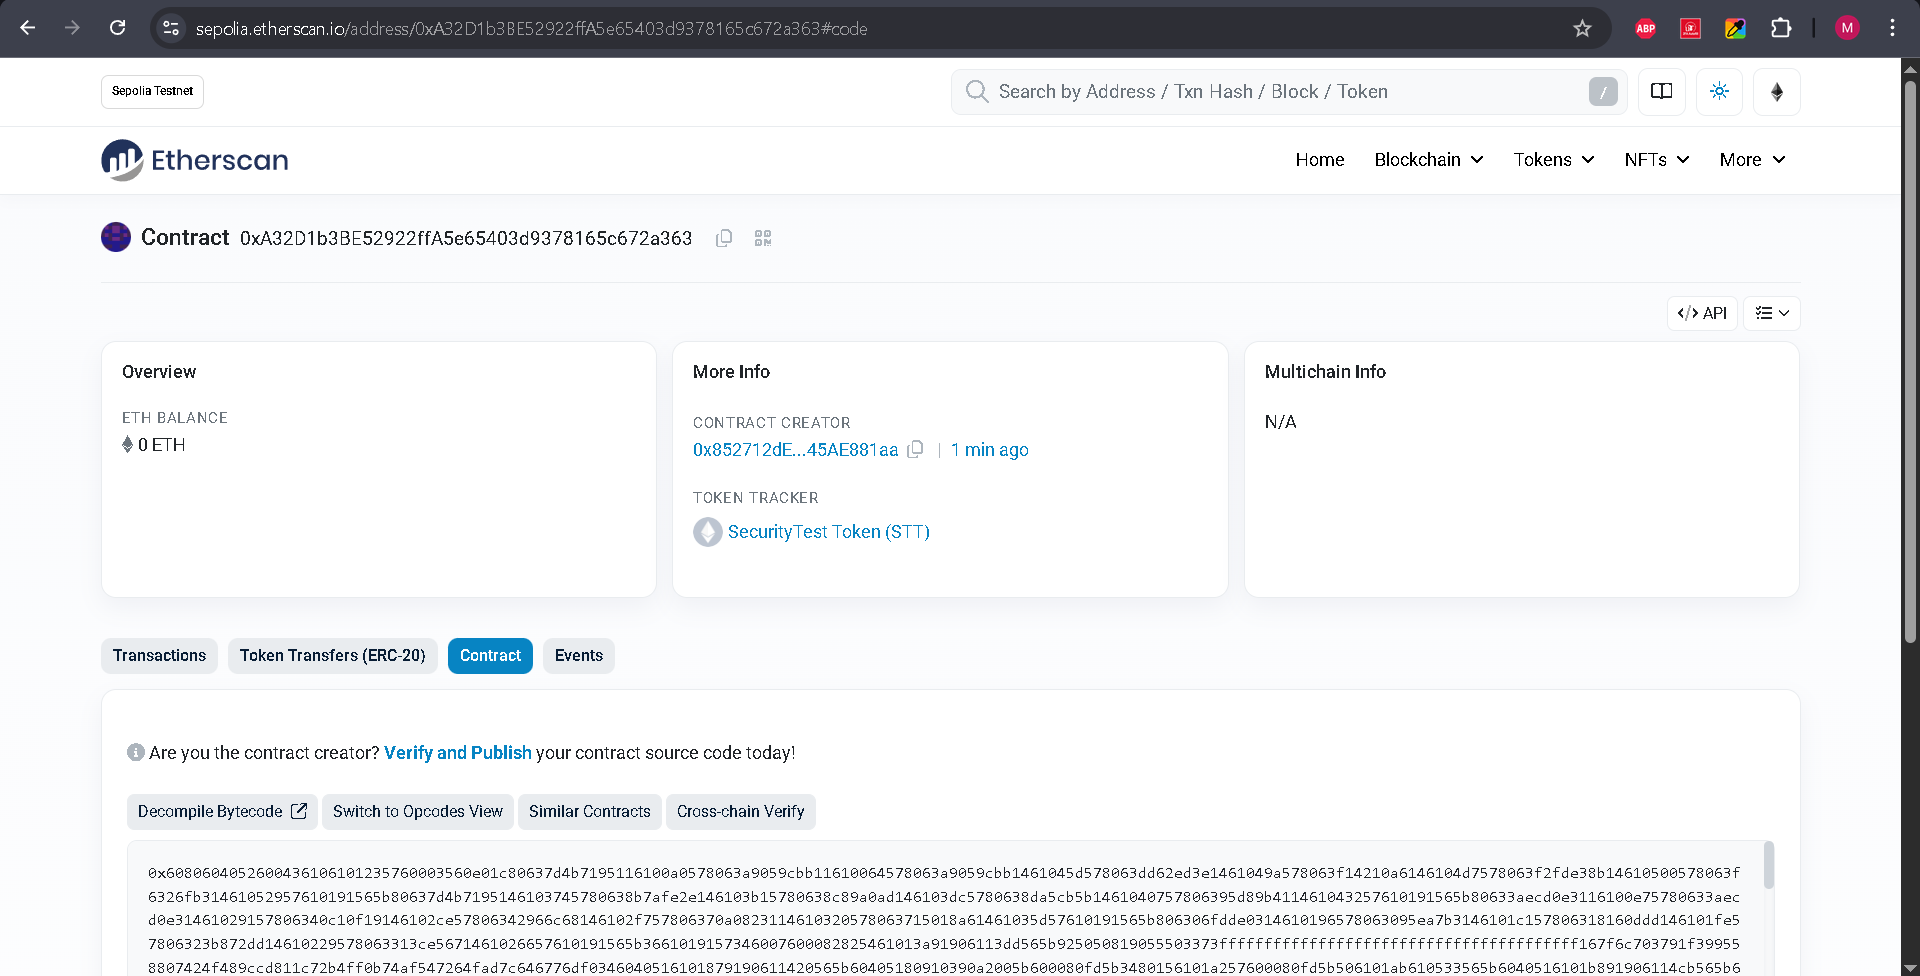
\includegraphics[width=\dimexpr\textwidth-2\fboxsep\relax]{imgs/primer_contrato.PNG}%
}
\caption{Contracte \texttt{SecurityTestContract} verificat a Etherscan sobre la xarxa Sepolia}
\label{fig:contract_verified}
\end{figure}


\subsubsection{Preparació de les operacions de prova}

A partir dels contractes desplegats es van preparar diferents operacions representatives per activar el flux d’anàlisi del sistema. Els escenaris principals inclouen aprovacions limitades, aprovacions molt elevades o pràcticament il·limitades, permisos globals mitjançant \texttt{setApprovalForAll(address,bool)} i operacions de dipòsit d’ETH.

En el cas de \texttt{SecurityTestContract}, els escenaris se centren en operacions associades a tokens fungibles, especialment aprovacions de despesa. La DApp pot construir manualment la \textit{calldata} corresponent a partir del selector de la funció i dels paràmetres codificats, cosa que permet generar transaccions controlades amb diferents nivells de risc.

En el cas de \texttt{SecurityTestNFT}, l’escenari principal és l’autorització global d’un operador mitjançant \texttt{setApprovalForAll(true)}. Aquesta operació és diferent d’una aprovació ERC20, ja que no autoritza una quantitat concreta de tokens, sinó la gestió de tots els NFTs de l’usuari dins d’una col·lecció. Per aquest motiu, el backend la tracta com un patró de risc específic quan el paràmetre \texttt{approved} és cert. En canvi, \texttt{setApprovalForAll(false)} es pot interpretar com una revocació del permís global.

Aquests escenaris constitueixen la base funcional sobre la qual es duen a terme les proves descrites posteriorment al Capítol~\ref{cap:evaluation}.

Una part de les operacions no es genera des de la DApp, sinó des de la pestanya \textit{Write Contract} d’Etherscan. Aquesta funcionalitat de l’explorador de blocs està disponible per a qualsevol contracte amb el codi font verificat i construeix un formulari a partir de l’ABI publicada: mostra la llista de funcions que modifiquen l’estat de la blockchain, un camp d’entrada per a cada paràmetre i un botó que prepara la transacció corresponent. Quan l’usuari confirma l’operació, Etherscan no la signa, sinó que la delega a la cartera connectada, que és qui demana la signatura final.

Aquest mecanisme té dos avantatges per a l’avaluació. D’una banda, permet invocar les funcions reals dels contractes desplegats sense escriure la \textit{calldata} manualment, ja que és el mateix explorador qui la codifica a partir dels valors introduïts. De l’altra, i més important, demostra que el sistema reacciona davant d’operacions iniciades des d’una eina externa i àmpliament utilitzada al sector, i no únicament des de la DApp construïda a mida per al projecte. La Figura~\ref{fig:write_contract} mostra aquesta interfície durant l’execució d’una operació sobre un dels contractes de prova.

\begin{figure}[H]
\centering
\colorbox{white}{%
    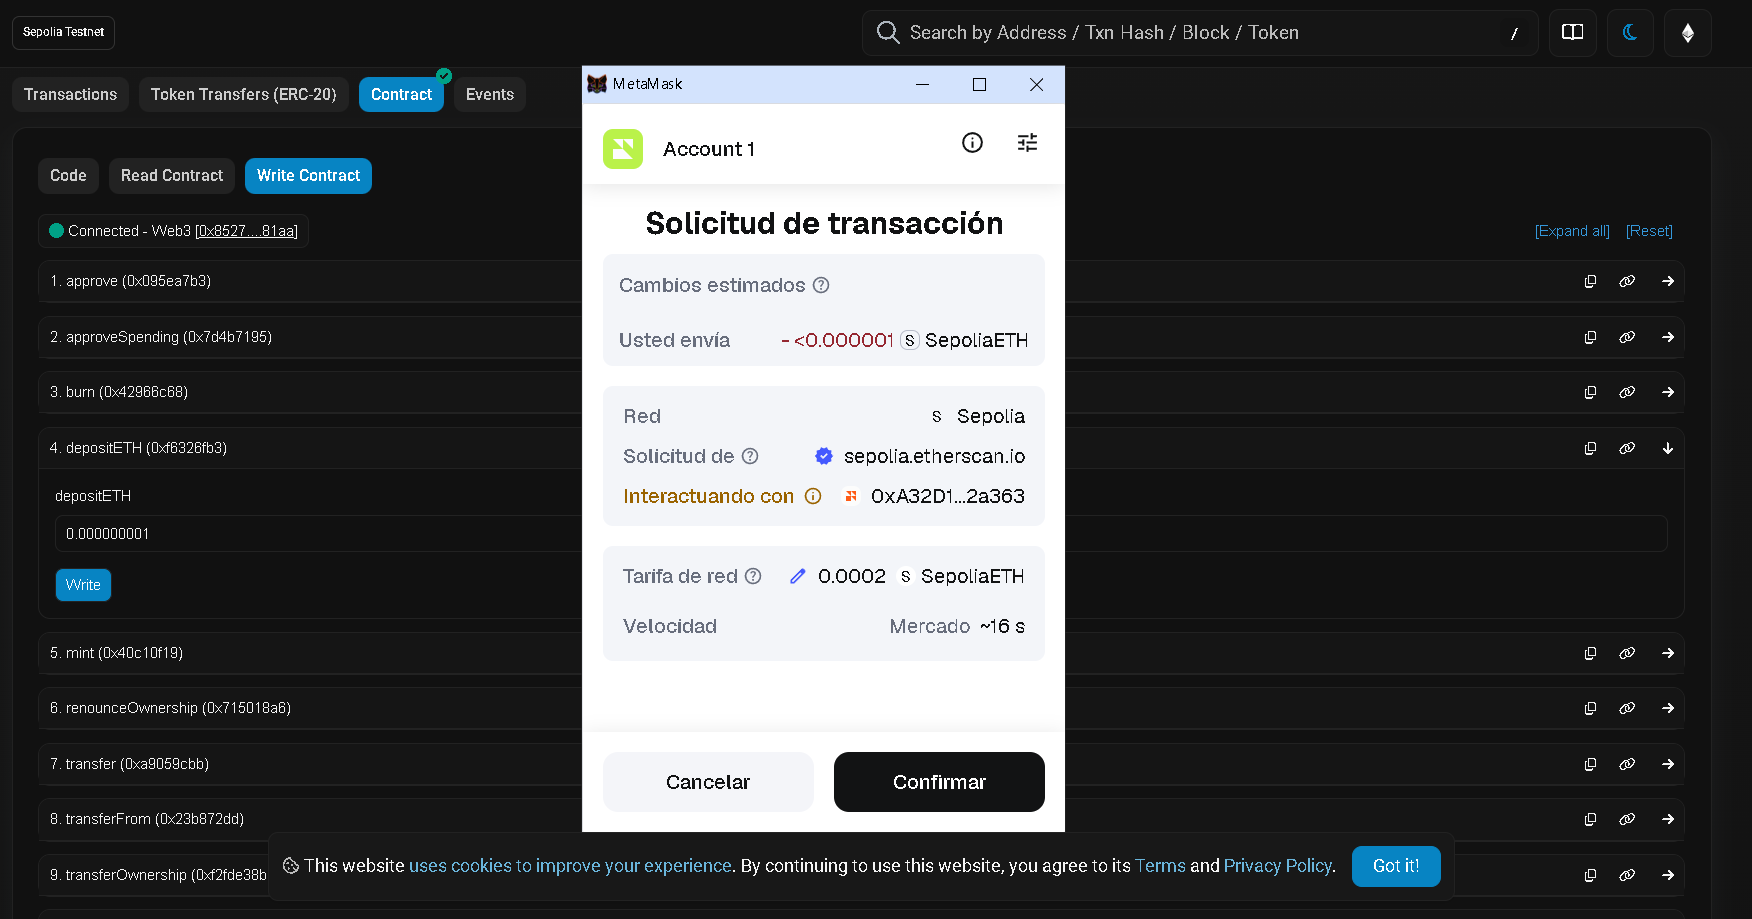
\includegraphics[width=\dimexpr\textwidth-2\fboxsep\relax]{imgs/depositar2_contrato1.PNG}%
}
\caption{Execució d’una operació sobre el contracte des de la interfície}
\label{fig:write_contract}
\end{figure}
